\documentclass[a4paper,11pt,twoside]{article}
%\documentclass[a4paper,11pt,twoside,se]{article}

\usepackage{UmUStudentReport}
\usepackage{verbatim}   % Multi-line comments using \begin{comment}
\usepackage{courier}    % Nicer fonts are used. (not necessary)
\usepackage{pslatex}    % Also nicer fonts. (not necessary)
\usepackage[pdftex]{graphicx}   % allows including pdf figures
\usepackage{listings}
\usepackage{pgf-umlcd}
%\usepackage{lmodern}   % Optional fonts. (not necessary)
%\usepackage{tabularx}
%\usepackage{microtype} % Provides some typographic improvements over default settings
%\usepackage{placeins}  % For aligning images with \FloatBarrier
%\usepackage{booktabs}  % For nice-looking tables
%\usepackage{titlesec}  % More granular control of sections.

% DOCUMENT INFO
% =============
\department{Department of Computing Science}
\coursename{Object-Oriented Programming Methodology 7.5 p}
\coursecode{5DV133}
\title{OU3 Sensor Network}
\author{Johan Eklund ({\tt{kv03jed@cs.umu.se}}) \\ 
Tommie Lindberg ({\tt{c15tlg@cs.umu.se}}) \\
Jakob Lundin ({\tt{c14jln@cs.umu.se}}) \\
Lorenz Gerber ({\tt{dv15lgr@cs.umu.se}}, {\tt{lozger03@student.umu.se}})
}
\date{2016-05-04}
%\revisiondate{2016-01-18}
\instructor{Anders Broberg \\ Niklas Fries \\ Adam Dahlgren \\
  Jonathan Westin \\ Erik Moström \\ Alexander Sutherland}


% DOCUMENT SETTINGS
% =================
\bibliographystyle{plain}
%\bibliographystyle{ieee}
\pagestyle{fancy}
\raggedbottom
\setcounter{secnumdepth}{2}
\setcounter{tocdepth}{2}
%\graphicspath{{images/}}   %Path for images

\usepackage{float}
\floatstyle{ruled}
\newfloat{listing}{thp}{lop}
\floatname{listing}{Listing}



% DEFINES
% =======
%\newcommand{\mycommand}{<latex code>}

% DOCUMENT
% ========
\begin{document}
\lstset{language=C}
\maketitle
\thispagestyle{empty}
\newpage
\tableofcontents
\thispagestyle{empty}
\newpage

\clearpage
\pagenumbering{arabic}

\section{Introduction} 
The assignment was described on the course homepage
\cite{sensornetwork}. 

\subsection{General Design Considerations}
It seems a reasonable approach to design the application as a model of a
real sensor network as described in Braginsky and Estrin
\cite{braginsky2002}. In particular should responsibilites
and collaborations somehow coincide with those of a real sensor
network. The realworld entities modelled in this assignment can be classified
in two groups: Physical components such as the sensor nodes and
information packages travelling the network, such as the queries and
the agents or specifically for the model. Further, is also a third
type, the environment entity which simulates the real surrounding.



\textit{Unified Modelling Language}
(\textit{UML}) and \textit{Class Responsibility Collaborator}
(\textit{CRC}) diagrams were composed according to Börstler
\cite{roleplay}. The theory of rumour routing is described by Braginsky
\cite{braginsky2002}. Horstman was used as Java language reference
\cite{horstman2014}.


\section{Classes Responsibilities and Collaborations}

\begin{figure}
\centering
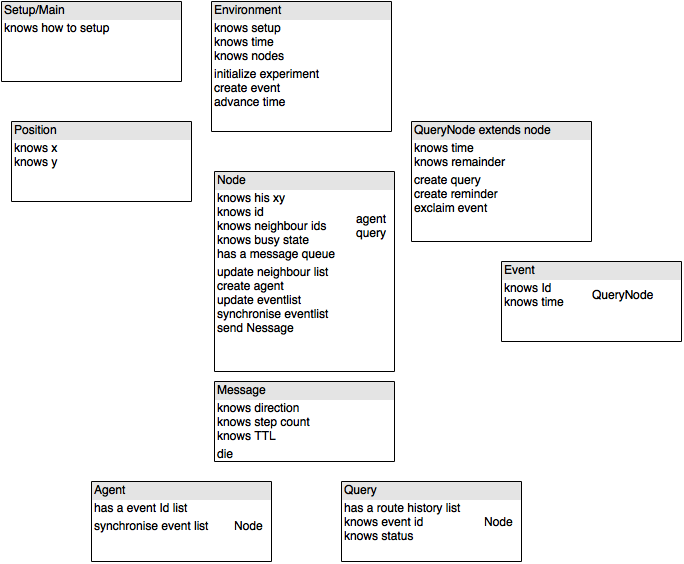
\includegraphics[width=\textwidth]{crc.png}
\caption{This is the crc diagram}
\label{fig:crc}
\end{figure}

\section{Unified Modelling Language Class Diagram}



\section{Initialization and State Stepping}
Parameters that are needed to create nodes have to be determined.
That includes the position, and the probability to create agents after
an event happens. 
Nodes have to be created and positioned. 
Nodes have to be initialized to know their neighbours
Experimental parameters for the environment have to be determined.
These include, which nodes will create queries. 


The nodes need to know their neighbours to become operational. To know
the neighbours, all nodes need to have a position. Either the
neighbours are just defined as a list, or a process that determines
the neighbours based on coordinates and sender/receiver range

\section{Testing Framework}


\addcontentsline{toc}{section}{\refname}
\bibliography{references}

\end{document}
 